%package list
\documentclass{article}
\usepackage[top=3cm, bottom=3cm, outer=3cm, inner=3cm]{geometry}
\usepackage{multicol}
\usepackage{graphicx}
\usepackage{url}
%\usepackage{cite}
\usepackage{hyperref}
\usepackage{array}
%\usepackage{multicol}
\newcolumntype{x}[1]{>{\centering\arraybackslash\hspace{0pt}}p{#1}}
\usepackage{natbib}
\usepackage{pdfpages}
\usepackage{multirow}
\usepackage[normalem]{ulem}
\useunder{\uline}{\ul}{}
\usepackage{svg}
\usepackage{xcolor}
\usepackage{listings}
\lstdefinestyle{ascii-tree}{
    literate={├}{|}1 {─}{--}1 {└}{+}1 
  }
\lstset{basicstyle=\ttfamily,
  showstringspaces=false,
  commentstyle=\color{red},
  keywordstyle=\color{blue}
}
%\usepackage{booktabs}
\usepackage{caption}
\usepackage{subcaption}
\usepackage{float}
\usepackage{array}

\newcolumntype{M}[1]{>{\centering\arraybackslash}m{#1}}
\newcolumntype{N}{@{}m{0pt}@{}}


%%%%%%%%%%%%%%%%%%%%%%%%%%%%%%%%%%%%%%%%%%%%%%%%%%%%%%%%%%%%%%%%%%%%%%%%%%%%
%%%%%%%%%%%%%%%%%%%%%%%%%%%%%%%%%%%%%%%%%%%%%%%%%%%%%%%%%%%%%%%%%%%%%%%%%%%%
\newcommand{\itemEmail}{aquispearr@unsa.edu.pe}
\newcommand{\itemEmail}{pcaril@unsa.edu.pe}
\newcommand{\itemEmail}{jbasurcoc@unsa.edu.pe}

\newcommand{\itemStudentA}{Alexandra Raquel Quispe   } 
\newcommand{\itemStudentB}{Paul Andree Cari                    } 
\newcommand{\itemStudentC}{Jeferson Joao Basurco} 

\newcommand{\itemCourse}{Programación Web II}
\newcommand{\itemCourseCode}{20231001}
\newcommand{\itemSemester}{I}
\newcommand{\itemUniversity}{Universidad Nacional de San Agustín de Arequipa}
\newcommand{\itemFaculty}{Facultad de Ingeniería de Producción y Servicios}
\newcommand{\itemDepartment}{Departamento Académico de Ingeniería de Sistemas e Informática}
\newcommand{\itemSchool}{Escuela Profesional de Ingeniería de Sistemas}
\newcommand{\itemAcademic}{2024 - A}
\newcommand{\itemInput}{Del 14 Mayo 2024}
\newcommand{\itemOutput}{Al 18 Mayo 2023}
\newcommand{\itemPracticeNumber}{04}
\newcommand{\itemTheme}{Ajax}
%%%%%%%%%%%%%%%%%%%%%%%%%%%%%%%%%%%%%%%%%%%%%%%%%%%%%%%%%%%%%%%%%%%%%%%%%%%%
%%%%%%%%%%%%%%%%%%%%%%%%%%%%%%%%%%%%%%%%%%%%%%%%%%%%%%%%%%%%%%%%%%%%%%%%%%%%

\usepackage[english,spanish]{babel}
\usepackage[utf8]{inputenc}
\AtBeginDocument{\selectlanguage{spanish}}
\renewcommand{\figurename}{Figura}
\renewcommand{\refname}{Referencias}
\renewcommand{\tablename}{Tabla} %esto no funciona cuando se usa babel
\AtBeginDocument{%
	\renewcommand\tablename{Tabla}
}

\usepackage{fancyhdr}
\pagestyle{fancy}
\fancyhf{}
\setlength{\headheight}{30pt}
\renewcommand{\headrulewidth}{1pt}
\renewcommand{\footrulewidth}{1pt}
\fancyhead[L]{\raisebox{-0.2\height}{
\includegraphics[width=3cm]{img/logo_episunsa.png}}}
\fancyhead[C]{\fontsize{7}{7}\selectfont	\itemUniversity \\ \itemFaculty \\ \itemDepartment \\ \itemSchool \\ \textbf{\itemCourse}}
\fancyhead[R]{\raisebox{-0.2\height}{
\includegraphics[width=1.2cm]{img/logo_abet}}}
\fancyfoot[L]{Quispe Alexandra - Cari Paul - Basurco Joao}
\fancyfoot[C]{\itemCourse}
\fancyfoot[R]{Página \thepage}

% para el codigo fuente
\usepackage{listings}
\usepackage{color, colortbl}
\definecolor{dkgreen}{rgb}{0,0.6,0}
\definecolor{gray}{rgb}{0.5,0.5,0.5}
\definecolor{mauve}{rgb}{0.58,0,0.82}
\definecolor{codebackground}{rgb}{0.95, 0.95, 0.92}
\definecolor{tablebackground}{rgb}{0.8, 0, 0}

\lstset{frame=tb,
	language=bash,
	aboveskip=3mm,
	belowskip=3mm,
	showstringspaces=false,
	columns=flexible,
	basicstyle={\small\ttfamily},
	numbers=none,
	numberstyle=\tiny\color{gray},
	keywordstyle=\color{blue},
	commentstyle=\color{dkgreen},
	stringstyle=\color{mauve},
	breaklines=true,
	breakatwhitespace=true,
	tabsize=3,
	backgroundcolor= \color{codebackground},
}

\begin{document}
	
	\vspace*{10px}
	
	\begin{center}	
		\fontsize{17}{17} \textbf{ Informe de Laboratorio \itemPracticeNumber}
	\end{center}
	\centerline{\textbf{\Large Tema: \itemTheme}}
	%\vspace*{0.5cm}	

	\begin{flushright}
		\begin{tabular}{|M{2.5cm}|N|}
			\hline 
			\rowcolor{tablebackground}
			\color{white} \textbf{Nota}  \\
			\hline 
			     \\[30pt]
			\hline 			
		\end{tabular}
	\end{flushright}	

	\begin{table}[H]
		\begin{tabular}{|x{4.7cm}|x{4.8cm}|x{4.8cm}|}
			\hline 
			\rowcolor{tablebackground}
			\color{white} \textbf{Estudiante} & \color{white}\textbf{Escuela}  & \color{white}\textbf{Asignatura}   \\
			\hline 
			{\itemStudentA 
   \itemStudentB
   \itemStudentC 
   \par } & \itemSchool & {\itemCourse \par Semestre: \itemSemester \par Código: \itemCourseCode}     \\
			\hline 			
		\end{tabular}
	\end{table}		
	
	\begin{table}[H]
		\begin{tabular}{|x{4.7cm}|x{4.8cm}|x{4.8cm}|}
			\hline 
			\rowcolor{tablebackground}
			\color{white}\textbf{Laboratorio} & \color{white}\textbf{Tema}  & \color{white}\textbf{Duración}   \\
			\hline 
			\itemPracticeNumber & \itemTheme & 12 horas   \\
			\hline 
		\end{tabular}
	\end{table}
	
	\begin{table}[H]
		\begin{tabular}{|x{4.7cm}|x{4.8cm}|x{4.8cm}|}
			\hline 
			\rowcolor{tablebackground}
			\color{white}\textbf{Semestre académico} & \color{white}\textbf{Fecha de inicio}  & \color{white}\textbf{Fecha de entrega}   \\
			\hline 
			\itemAcademic & \itemInput &  \itemOutput  \\
			\hline 
		\end{tabular}
	\end{table}
	
	\section{Tarea}
	\begin{itemize}		
Para la tarea sobre Ajax en w3schools, se debe revisar la sección correspondiente en dicho sitio web y presentar un informe con capturas de pantalla de cada ejemplo de Ajax implementado en su propio servidor web.

Además, se requiere realizar una práctica utilizando Ajax y Google Charts. Primero, es necesario instalar Python en la computadora y lanzar un servidor web local utilizando los comandos:
\begin{verbatim}
python -m SimpleHTTPServer 8000  # Para Python 2
python3 -m http.server 8000       # Para Python 3
\end{verbatim}
Alternativamente, se puede utilizar un servidor web como Apache con Xampp. Luego, se debe descargar el archivo \texttt{data.json} y colocarlo en el directorio raíz del servidor web.

Para cada problema propuesto, se debe implementar un programa en Ajax y una página que realice las siguientes tareas:
\begin{itemize}
    \item Listar todas las regiones.
    \item Mostrar el número total de confirmados por región.
    \item Encontrar las 10 regiones con mayor número de confirmados.
    \item Visualizar un gráfico temporal de los valores para Arequipa.
    \item Crear gráficos comparativos entre regiones usando líneas.
    \item Visualizar un gráfico del crecimiento en regiones, excluyendo Lima y Callao.
    \item Realizar gráficos comparativos entre regiones elegidas por el usuario.
    \item Mostrar un gráfico comparativo del crecimiento diario en regiones, excluyendo Lima y Callao.
\end{itemize}
	\end{itemize}
		
\section{Equipos, materiales y temas utilizados}
\begin{itemize}
    \item \textbf{Sistema Operativo:} Ubuntu GNU/Linux 23.04 Lunar Lobster 64 bits, Kernel 6.2.
    \item \textbf{Editor de texto:} VIM 9.0.
    \item \textbf{Entorno de desarrollo:} OpenJDK 64-Bits 17.0.7.
    \item \textbf{Control de versiones:} Git 2.39.2.
    \item \textbf{Repositorio:} Cuenta en GitHub con el correo institucional.
    \item \textbf{Tecnologías utilizadas:}
    \begin{itemize}
        \item \textbf{Ajax:} Para la implementación de solicitudes asíncronas y la manipulación dinámica de datos.
        \item \textbf{Google Charts:} Para la visualización gráfica de datos, incluyendo gráficos de líneas y gráficos comparativos.
        \item \textbf{Python:} Utilizado para lanzar un servidor web local para pruebas.
        \item \textbf{Servidor web:} SimpleHTTPServer (Python 2) o http.server (Python 3) para el desarrollo y prueba de aplicaciones web.
    \end{itemize}
\end{itemize}

\section{URL de Repositorio GitHub}
\begin{itemize}
    \item URL del Repositorio GitHub para clonar o recuperar.
    \item \url{https://github.com/JefersonPWeb2/Pw2-Lab04.git}
    \item URL de los videos explicativos de cada integrante.
    \item \url{https://docs.google.com/document/d/1frXNSmf9j4nQTG4MYFCRL4iT6l_N5MXCwpCSuqlvZPM/edit?usp=sharing}
\end{itemize}

\section{Actividades con el repositorio GitHub}

\subsection{Tarea Ajax en w3schools}


\begin{itemize}
    \item Capturas W3schools AJAX.
    \item \url{https://docs.google.com/document/d/1mWWgP6RKmzeaMjWebnFMSfqGnqmgGHWAhDCAF-BAftk/edit}
\end{itemize}


\subsection{Tarea Ajax y NodeJS}

\begin{figure}[h]
    \centering
    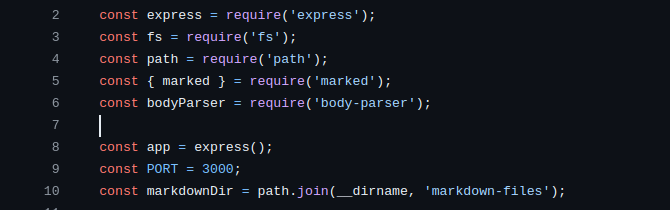
\includegraphics[width=0.9\linewidth]{latex//img/3.1.png}
    \caption{Configuración del servidor web en Node.js}
    \label{fig:import-modules}
\end{figure}

En esta tarea, utilizamos Node.js para configurar un servidor web con varios módulos esenciales. El código que se muestra en la Figura \ref{fig:import-modules} importa los siguientes módulos:
\begin{itemize}
    \item \textbf{express:} Utilizado para crear y gestionar el servidor web.
    \item \textbf{fs:} Proporciona funciones para interactuar con el sistema de archivos.
    \item \textbf{path:} Facilita la manipulación de rutas de archivos.
    \item \textbf{marked:} Convierte texto en formato Markdown a HTML.
    \item \textbf{body-parser:} Procesa los datos de las solicitudes HTTP.
\end{itemize}

El código crea una instancia de una aplicación Express, define el puerto del servidor como 3000 y especifica el directorio donde se almacenarán los archivos Markdown.



\begin{figure}[h]
    \centering
    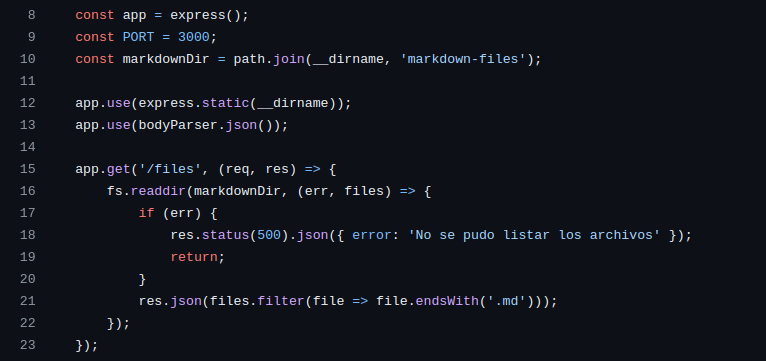
\includegraphics[width=0.9\linewidth]{latex//img/3.2.png}
    \caption{Configuración del servidor y manejo de solicitudes en Node.js}
    \label{fig:server-setup}
\end{figure}

El código en la Figura \ref{fig:server-setup} continúa con la configuración del servidor Node.js. Las siguientes líneas de código realizan estas acciones:
\begin{itemize}
    \item \textbf{Líneas 8-10:} Se inicializa la aplicación Express, se define el puerto del servidor como 3000 y se establece la ruta para almacenar los archivos Markdown.
    \item \textbf{Líneas 12-13:} Se configuran los archivos estáticos para ser servidos desde el directorio actual y se permite que el servidor analice las solicitudes en formato JSON.
    \item \textbf{Líneas 15-23:} Se maneja las solicitudes a la ruta \texttt{/files}, leyendo el contenido del directorio \texttt{markdownDir} y devolviendo una lista de los archivos que terminan en \texttt{.md}.
\end{itemize}






\subsubsection{Manejo de la solicitud para leer un archivo Markdown}
\begin{figure}[h]
    \centering
    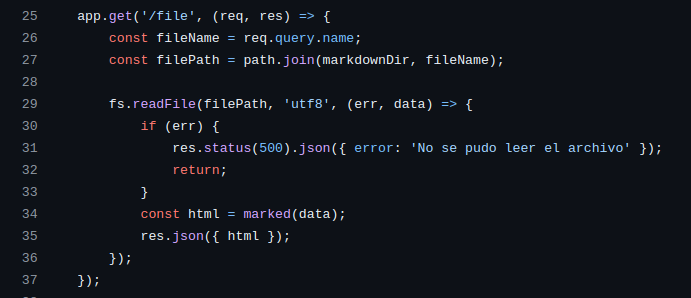
\includegraphics[width=0.9\linewidth]{latex//img/3.3.png}
    \caption{Lectura y conversión de archivos Markdown en Node.js}
    \label{fig:read-markdown-file}
\end{figure}

El código en la Figura \ref{fig:read-markdown-file} define una ruta que permite leer y convertir archivos Markdown a HTML. Las acciones específicas realizadas son:
\begin{itemize}
    \item La ruta \texttt{/file} toma el nombre del archivo desde la solicitud (\texttt{req.query.name}).
    \item Se construye la ruta completa del archivo utilizando \texttt{path.join(markdownDir, fileName)}.
    \item El archivo se lee en formato UTF-8 utilizando \texttt{fs.readFile}.
    \item Si ocurre un error durante la lectura, se devuelve un mensaje de error con el código de estado 500.
    \item Si la lectura es exitosa, el contenido del archivo se convierte a HTML usando \texttt{marked}.
    \item El HTML generado se devuelve como una respuesta JSON.
\end{itemize}




\subsubsection{Manejo de la solicitud para crear un archivo Markdown}
\begin{figure}[h]
    \centering
    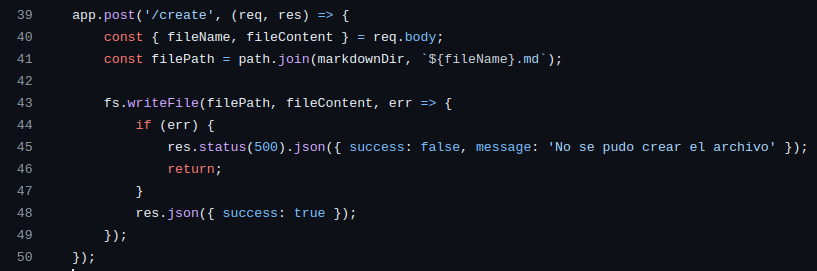
\includegraphics[width=0.9\linewidth]{latex//img/3.4.png}
    \caption{Creación de archivos Markdown en Node.js}
    \label{fig:create-markdown-file}
\end{figure}

El código en la Figura \ref{fig:create-markdown-file} define una ruta que permite crear nuevos archivos Markdown. Las acciones específicas realizadas son:
\begin{itemize}
    \item La ruta \texttt{/create} toma el nombre del archivo y su contenido desde el cuerpo de la solicitud (\texttt{req.body}).
    \item Se construye la ruta completa del archivo utilizando \texttt{path.join(markdownDir, `${fileName}.md`)}.
    \item El archivo se escribe utilizando \texttt{fs.writeFile}.
    \item Si ocurre un error durante la escritura, se devuelve un mensaje de error con el código de estado 500 y un indicador de éxito falso.
    \item Si la escritura es exitosa, se devuelve una respuesta JSON indicando éxito.
\end{itemize}





\subsubsection{Iniciando el servidor Node.js}
\begin{figure}[h]
    \centering
    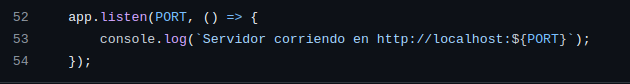
\includegraphics[width=0.9\linewidth]{latex//img/3.5.png}
    \caption{Iniciando el servidor en Node.js}
    \label{fig:start-server}
\end{figure}

El código en la Figura \ref{fig:start-server} inicia el servidor Node.js en el puerto 3000. Las acciones específicas realizadas son:
\begin{itemize}
    \item La función \texttt{app.listen(PORT)} inicia el servidor en el puerto especificado (3000 en este caso).
    \item Se muestra un mensaje en la consola indicando que el servidor está corriendo en \texttt{http://localhost:3000}.
\end{itemize}

\subsubsection{Estructura de carpetas del proyecto}
\begin{figure}[h]
    \centering
    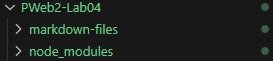
\includegraphics[width=0.5\linewidth]{latex//img/3.6.png}
    \caption{Estructura de carpetas del proyecto}
    \label{fig:folder-structure}
\end{figure}

En la Figura \ref{fig:folder-structure} se muestra la distribución de carpetas del proyecto Node.js. La carpeta \texttt{markdown-files} se crea para almacenar archivos con extensión ".md", mientras que la carpeta \texttt{node_modules} es una carpeta predeterminada generada al instalar las dependencias del proyecto, como Express, Marked y Body-parser.

\begin{figure}[h]
    \centering
    
\includegraphics[width=0.8\linewidth]{latex//img/3.7.png}
    \caption{Archivos en el proyecto}
    \label{fig:files-in-project-1}
        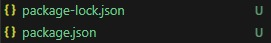
\includegraphics[width=0.5\linewidth]{latex//img/3.8.png}
    \caption{Archivos en el proyecto}
    \label{fig:files-in-project-2}
\end{figure}
Además, se crean automáticamente los archivos "package-lock.json" y "package.json" como parte de la configuración del proyecto.
\clearpage



\subsection{Tarea Ajax y Google Charts}
        \begin{itemize}	
		\item  Liste todas las “regiones”.
            \end{itemize}
         \lstinputlisting[language=JavaScript, caption={}, label={lst:codigo-js}]{list_regions.js}
         \lstinputlisting[language=HTML, caption={}, label={lst:ejemplo-html}]{list_regions.html}


         
         \subsection{Actividad}
        \begin{itemize}	
		\item  Muestre el número total de confirmados por región
            \end{itemize}
         \lstinputlisting[language=JavaScript, caption={}, label={lst:codigo-js}]{total_confirmed.js}
         \lstinputlisting[language=HTML, caption={}, label={lst:ejemplo-html}]{total_confirmed.html}
         
         \subsection{Actividad}
        \begin{itemize}	
		\item  Encuentre las 10 regiones cuya suma total sea la mayor
            \end{itemize}
         \lstinputlisting[language=JavaScript, caption={}, label={lst:codigo-js}]{top_regions.js}
         \lstinputlisting[language=HTML, caption={}, label={lst:ejemplo-html}]{top_regions.html}
         
         \subsection{Actividad}
        \begin{itemize}	
		\item  Visualice un gráfico en el tiempo de los valores para la región de Arequipa
            \end{itemize}
         \lstinputlisting[language=JavaScript, caption={}, label={lst:codigo-js}]{aqp_chart.js}
         \lstinputlisting[language=HTML, caption={}, label={lst:ejemplo-html}]{aqp_chart.html}

         \subsection{Actividad}
        \begin{itemize}	
		\item  Haga gráficos comparativos entre regiones usando líneas
            \end{itemize}
        \lstinputlisting[language=JavaScript, caption={}, label={lst:codigo-js}]{compare_regions.js}
         \lstinputlisting[language=HTML, caption={}, label={lst:ejemplo-html}]{compare_regions.html}

         \subsection{Actividad}
        \begin{itemize}	
		\item  Visualice un gráfico comparativo del crecimiento en regiones excepto Lima y Callao
            \end{itemize}
         \lstinputlisting[language=JavaScript, caption={}, label={lst:codigo-js}]{Lima.js}
        \lstinputlisting[language=HTML, caption={}, label={lst:ejemplo-html}]{Lima.html}

         \subsection{Actividad}
        \begin{itemize}	
		\item  Haga gráficos comparativos entre regiones elegidas por el usuario.
            \end{itemize}
         \lstinputlisting[language=JavaScript, caption={}, label={lst:codigo-js}]{comparativo.js}
         \lstinputlisting[language=HTML, caption={}, label={lst:ejemplo-html}]{comparativo.html}

         \subsection{Actividad}
        \begin{itemize}	
		\item  Visualice un gráfico comparativo del crecimiento en regiones excepto Lima y Callao, mostrando el número de confirmados por cada día
            \end{itemize}
         \lstinputlisting[language=JavaScript, caption={}, label={lst:codigo-js}]{regiones.js}
         \lstinputlisting[language=HTML, caption={}, label={lst:ejemplo-html}]{regiones.html}
  \clearpage  

\subsubsection{Capturas del funcionamiento}
\begin{figure}[h]
\centering
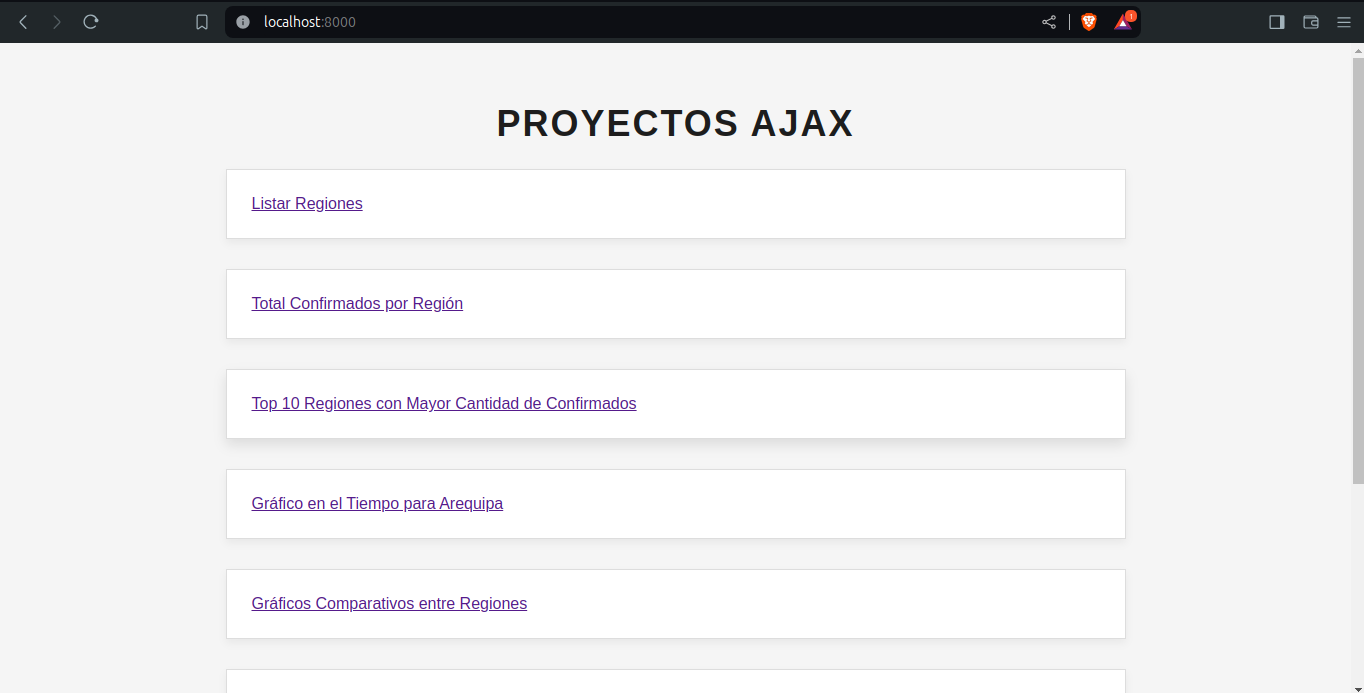
\includegraphics[width=0.8\linewidth]{latex//img/index_html.png}
\caption{}
\label{fig:enter-label}
\end{figure}
\begin{figure}[h]
\centering
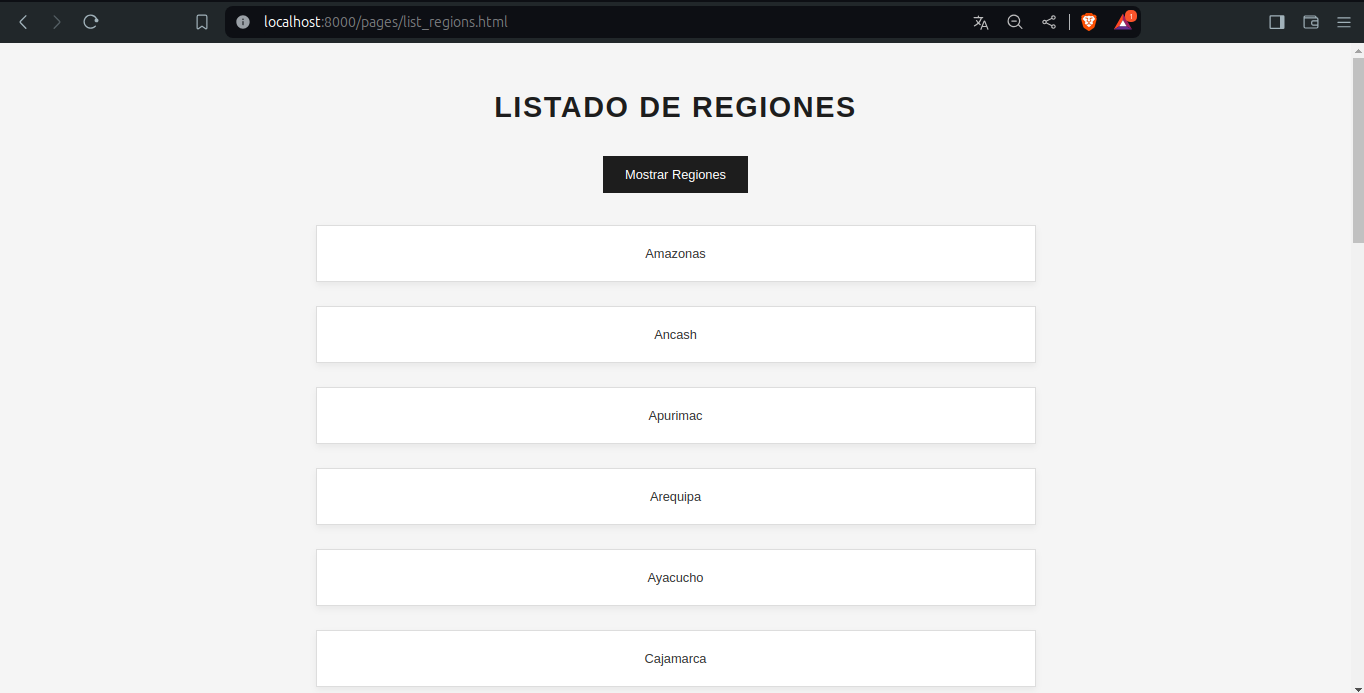
\includegraphics[width=0.8\linewidth]{latex//img/result2.png}
\caption{}
\label{fig:enter-label}
\end{figure}
\begin{figure}[h]
\centering
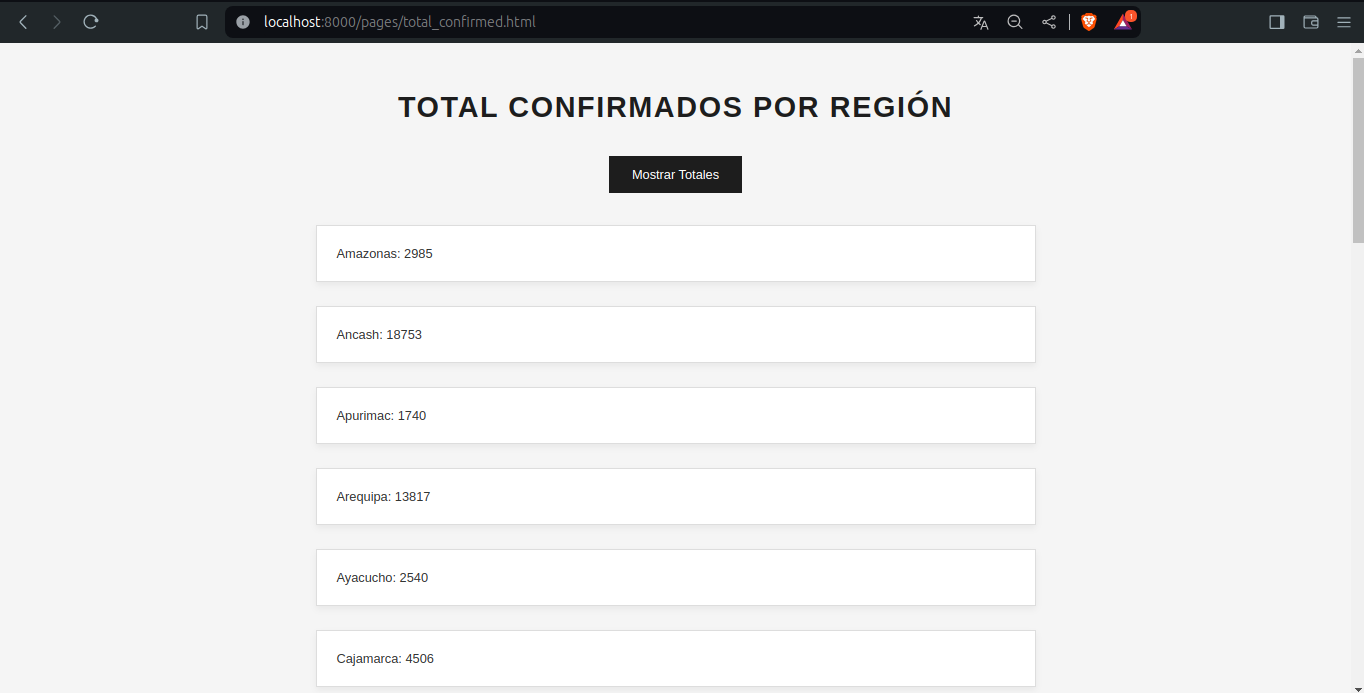
\includegraphics[width=0.8\linewidth]{latex//img/result3.png}
\caption{}
\label{fig:enter-label}
\end{figure}
\begin{figure}[h]
\centering
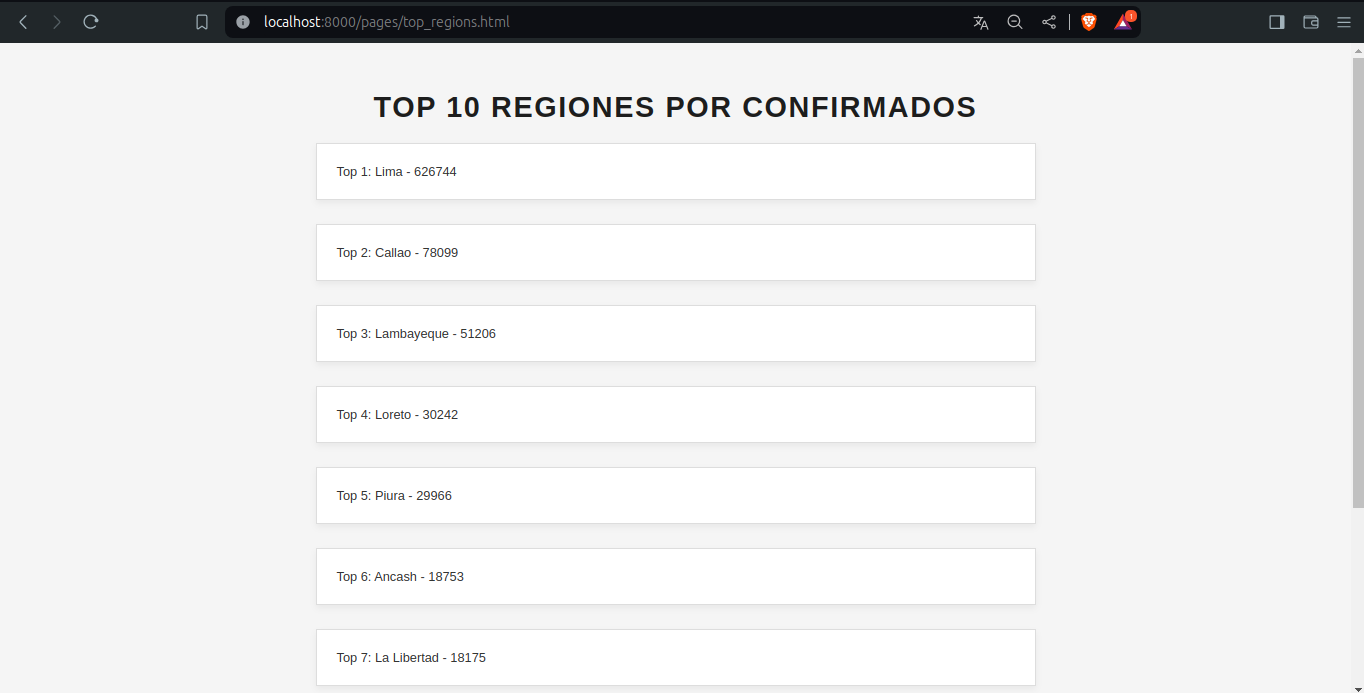
\includegraphics[width=0.75\linewidth]{latex//img/result4.png}
\caption{}
\label{fig:enter-label}
\end{figure}
\begin{figure}[h]
\centering
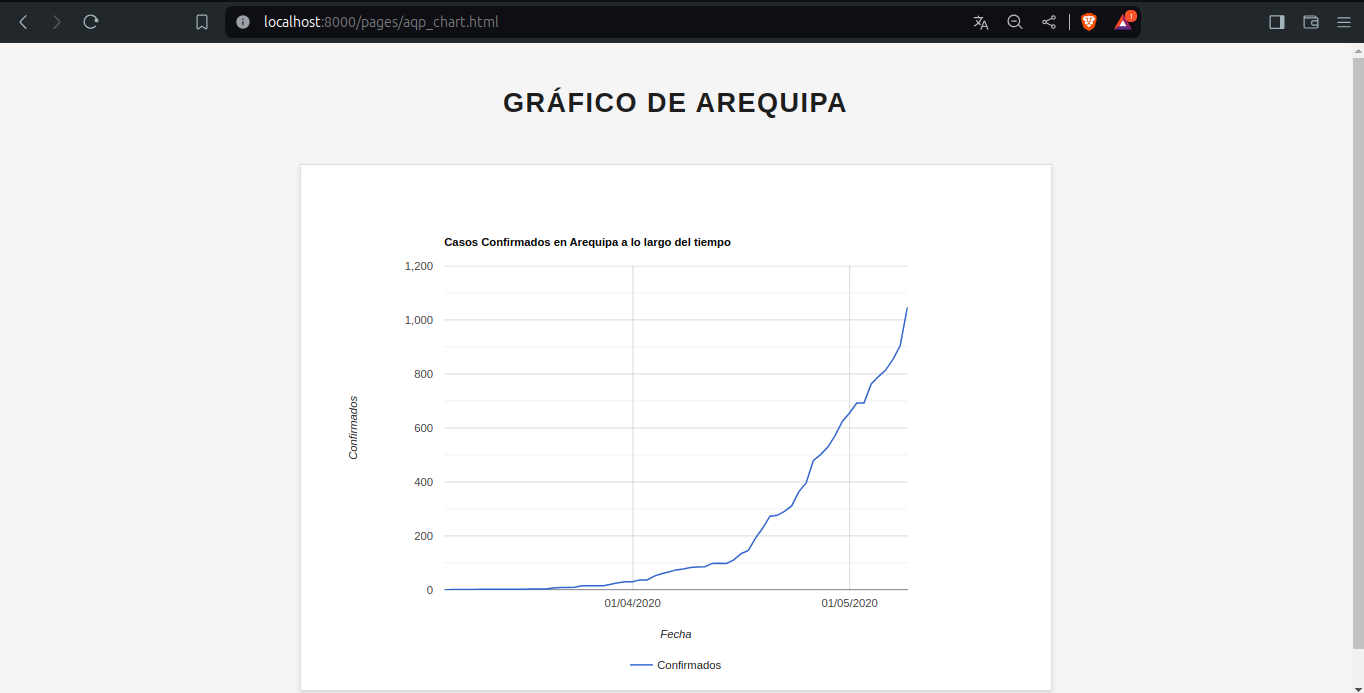
\includegraphics[width=0.75\linewidth]{latex//img/result5.png}
\caption{}
\label{fig:enter-label}
\end{figure}
\begin{figure}[h]
\centering
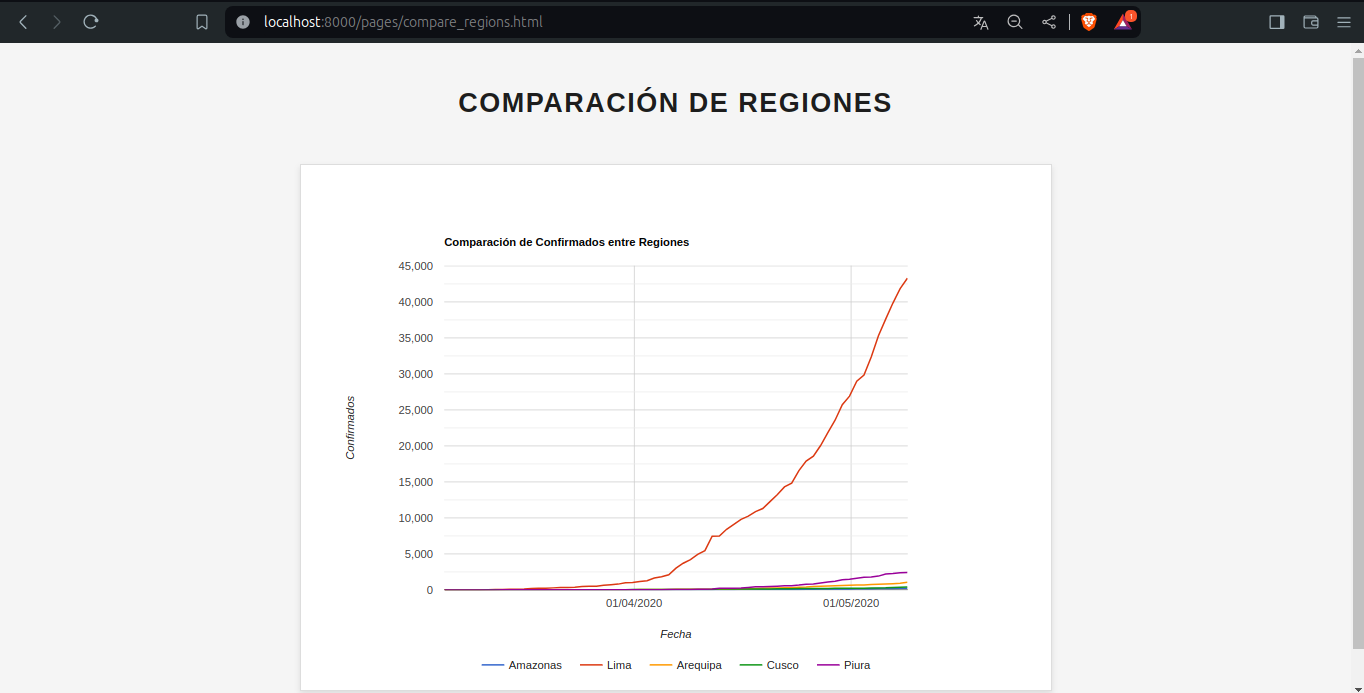
\includegraphics[width=0.75\linewidth]{latex//img/result6.png}
\caption{}
\label{fig:enter-label}
\end{figure}
\begin{figure}[h]
\centering
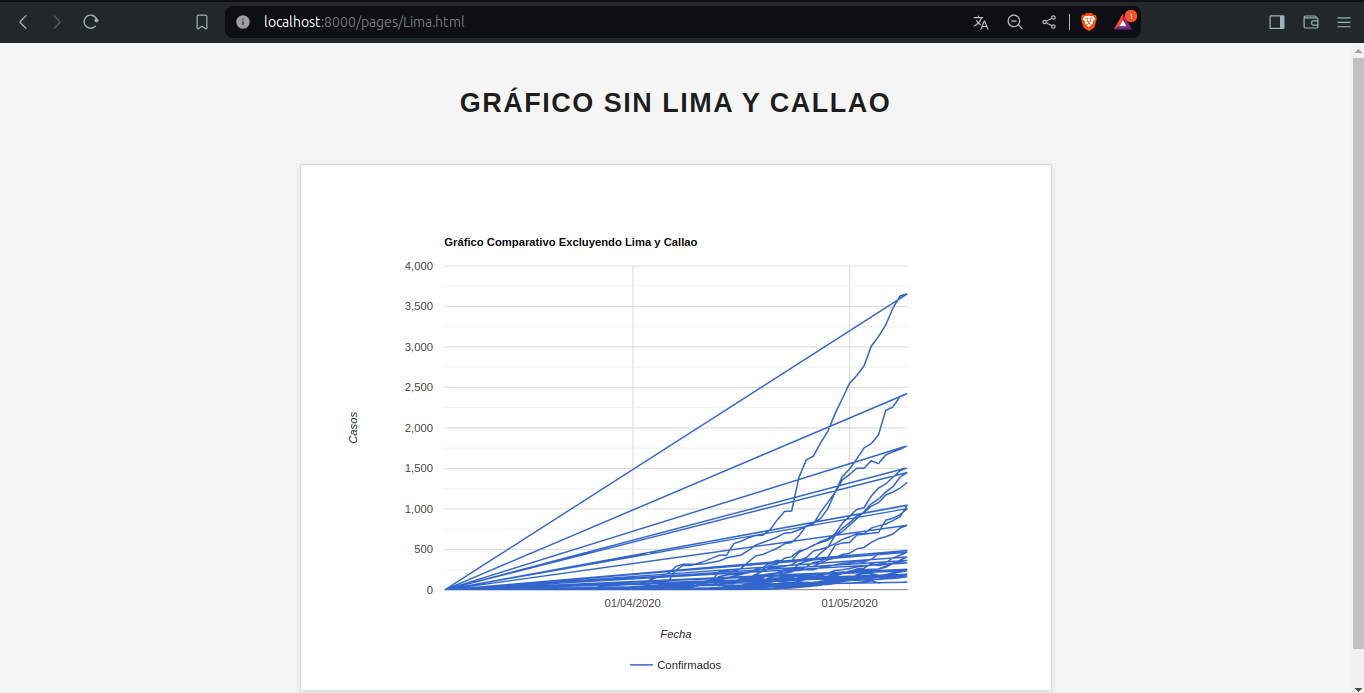
\includegraphics[width=0.75\linewidth]{latex//img/result7.png}
\caption{}
\label{fig:enter-label}
\end{figure}
\begin{figure}[h]
\centering
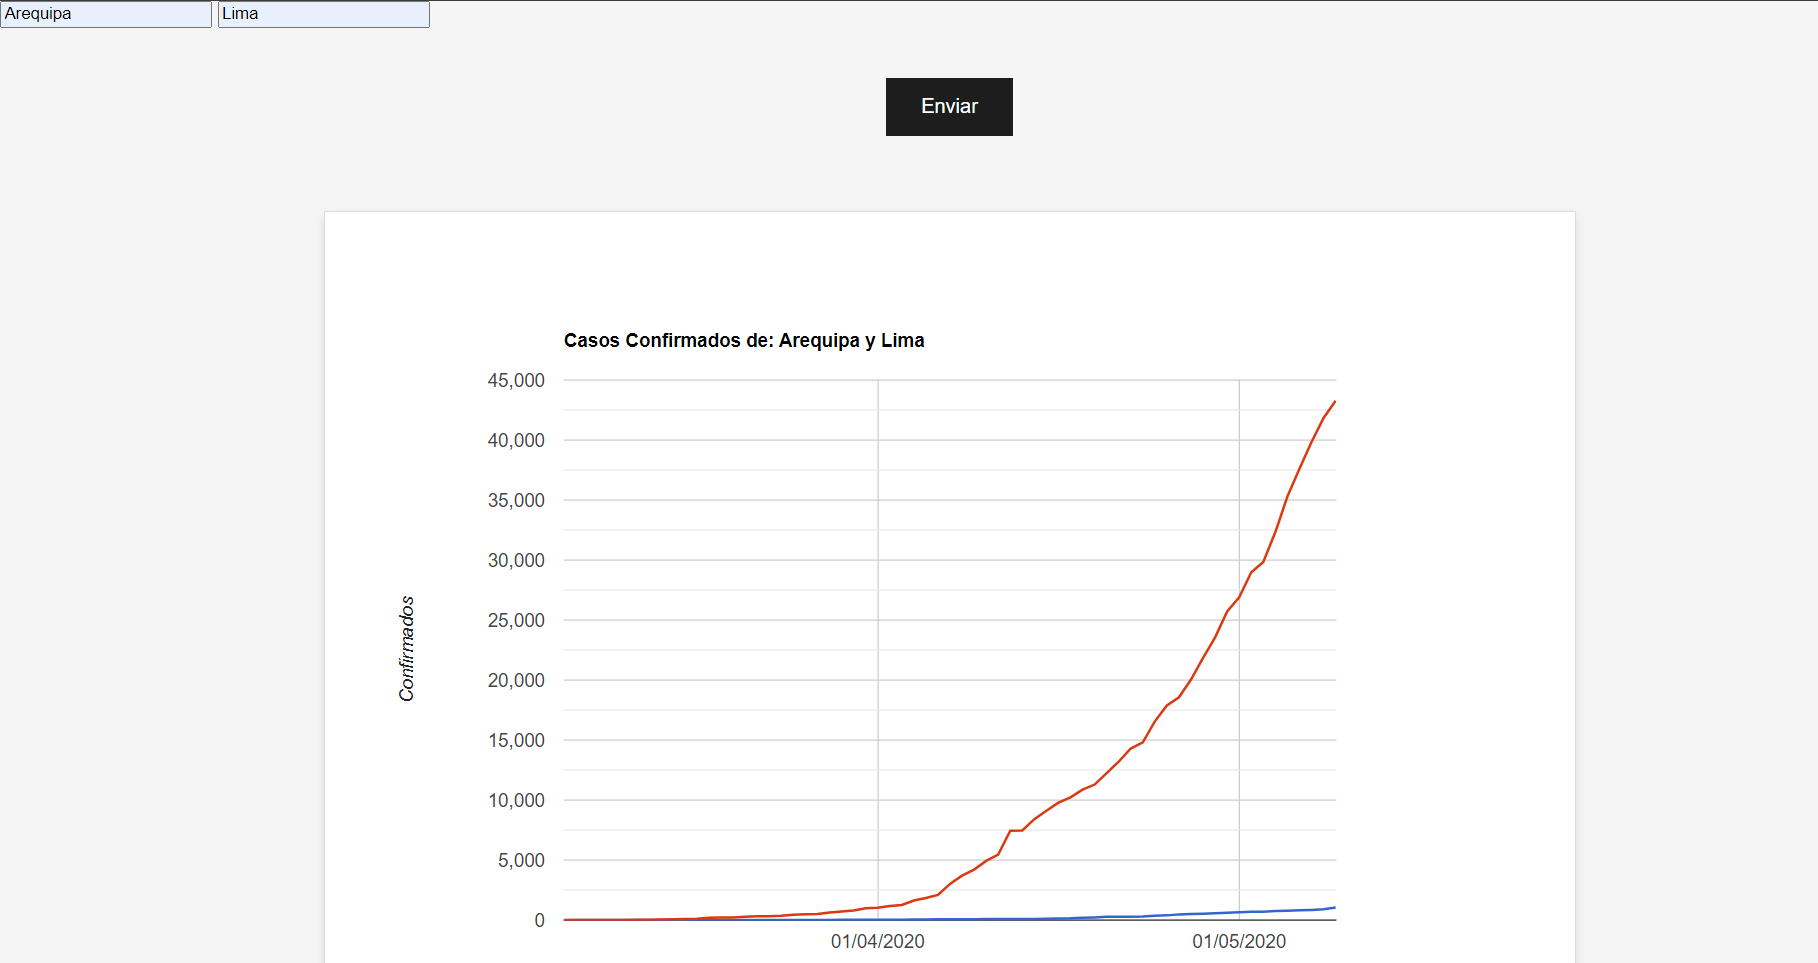
\includegraphics[width=0.75\linewidth]{latex/penultima.png}
\caption{}
\label{fig:enter-label}
\end{figure}
\begin{figure}[h]
\centering
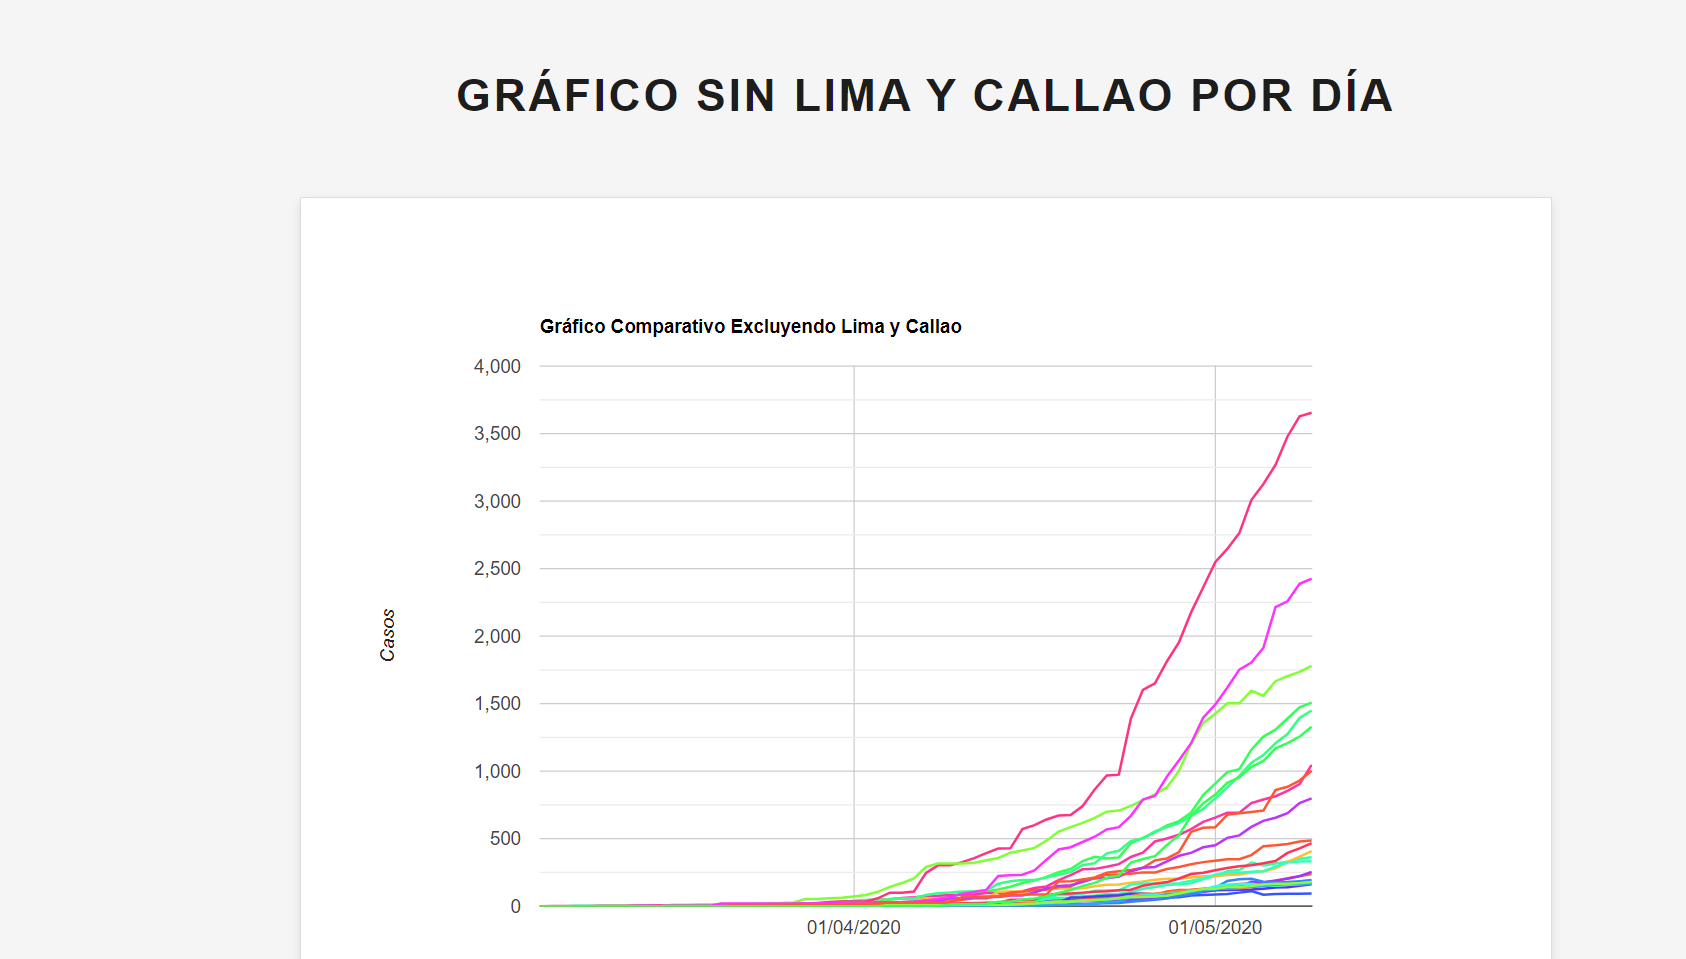
\includegraphics[width=0.75\linewidth]{latex/ultima.png}
\caption{}
\label{fig:enter-label}
\end{figure}



%%%%%%%%%%%%%%%%%%%%%%%%%%%%%%%%%%%%%%%%%%%%%%%%%%%%%%%%%%%%%%%%%%%%%%%%%%%%%%%%%%%%%%%%%%%%%%%%%%%%%%%%%
%%%%%%%%%%%%%%%%%%%%%%%%%%%%%%%%%%%		


	

			
\end{document}